\begin{figure}[htbp]
  \centering
  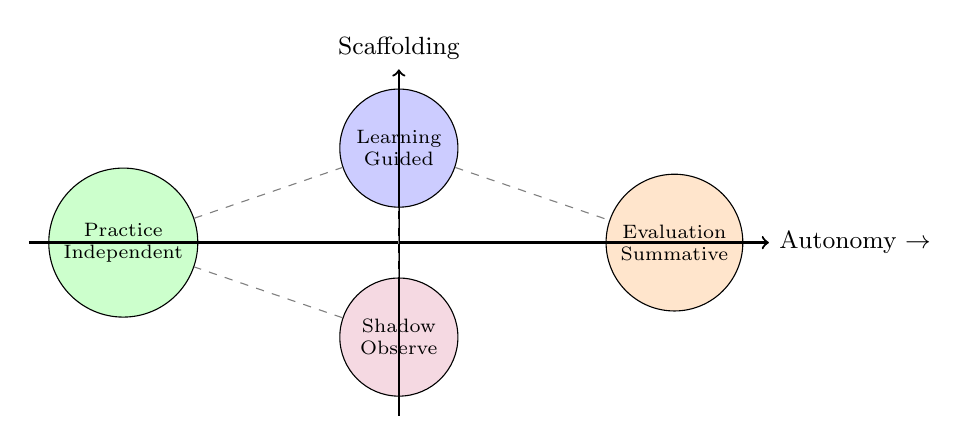
\begin{tikzpicture}[
    mode/.style={circle, draw, minimum size=1.5cm, font=\scriptsize, align=center},
    axis/.style={->, thick}
  ]
    \node[mode, fill=green!20] (p) at (0,0) {Practice\\Independent};
    \node[mode, fill=blue!20] (l) at (3.5,1.2) {Learning\\Guided};
    \node[mode, fill=orange!20] (e) at (7,0) {Evaluation\\Summative};
    \node[mode, fill=purple!15] (s) at (3.5,-1.2) {Shadow\\Observe};
    \draw[axis] (-1.2,0) -- (8.2,0) node[right,font=\small] {Autonomy $\rightarrow$};
    \draw[axis] (3.5,-2.2) -- (3.5,2.2) node[above,font=\small] {Scaffolding};
    \draw[dashed, gray] (p) -- (l);
    \draw[dashed, gray] (l) -- (e);
    \draw[dashed, gray] (s) -- (l);
    \draw[dashed, gray] (s) -- (p);
  \end{tikzpicture}
  \caption{Pedagogical positioning of MedPrep modes along scaffolding vs.\ learner autonomy axes.}
  \label{fig:mode-pedagogy}
\end{figure}
